\documentclass[conference]{IEEEtran}
\IEEEoverridecommandlockouts

\usepackage{cite}
\usepackage{amsmath,amssymb,amsfonts}
\usepackage{algorithm}
\usepackage{algorithmic}
\usepackage{graphicx}
\usepackage{textcomp}
\usepackage{xcolor}
\usepackage{booktabs}
\usepackage{xeCJK}
\setCJKmainfont{SimSun}

\begin{document}

\title{三维Voronoi自适应覆盖与动态边界追踪的水下溢油监测方法}

\author{\IEEEauthorblockN{作者姓名}
\IEEEauthorblockA{\textit{单位名称}\\
城市，国家\\
email@example.com}}

\maketitle

\begin{abstract}
水下溢油持续泄漏形成的污染羽流具有三维空间扩散、浓度分布高度非均匀以及边界动态扩张等特征。在有限感知半径条件下，传统基于密度加权质心反馈的多自主水下航行器覆盖方法极易陷入“集群塌陷”困境，即所有AUV向浓度峰值区域聚集，导致外部扩散边界丧失监测能力。针对上述问题，本文提出一种融合三维Voronoi自适应覆盖与动态边界追踪的多AUV协同监测方法。首先，建立考虑主流输运、各向异性湍流扩散、油滴浮力上升及自然衰减的持续泄漏三维高斯羽流模型，通过时间卷积积分刻画历史释放油团的累积效应。其次，将浓度场映射为时变覆盖密度函数，在三维有界水域中构造基于欧氏距离的体积Voronoi划分。进一步地，通过动态边界采样与空间均衡分配机制，设计包含质心反馈、质心速度前馈、边界追踪和分散项的控制律。仿真实验表明，标准CVT出现明显集群塌陷，最终动态覆盖率仅为38.24\%，边界追踪RMSE为66.75 m；相比之下，所提方法将动态覆盖率提升至58.86\%，并将边界追踪RMSE降低至15.94 m，同时满足AUV速度约束。实验验证了所提方法在三维动态溢油监测中的有效性。
\end{abstract}

\begin{IEEEkeywords}
水下溢油监测；多AUV协同；三维Voronoi覆盖；动态边界追踪；持续泄漏羽流；集群塌陷
\end{IEEEkeywords}

\section{引言}
水下溢油泄漏是海洋环境安全和海上工程运行中的重要风险源。与水面溢油相比，水下泄漏污染物在海流输运、湍流扩散、浮力上升和自然衰减等因素共同作用下形成三维时变羽流，其空间结构复杂、浓度分布高度非均匀，并且污染边界随时间持续扩张。已有研究表明，泄漏速率和海流速度会显著影响水下溢油的迁移路径和扩散范围\cite{zhang2020oil}，溢油建模也需要综合考虑输运、扩散和衰减等物理过程\cite{fingas2022overview}。

自主水下航行器具有三维机动、自主导航和近距离感知能力，适合执行水下污染监测和应急巡检任务。多AUV协同监测的关键在于如何根据污染浓度分布动态调整空间位置，使有限数量的智能体既能覆盖高浓度核心区域，又能持续跟踪污染羽流的外部边界。经典覆盖控制方法通常基于Voronoi划分和位置感知代价函数建立\cite{cortes2004coverage}，并通过Lloyd迭代或质心反馈驱动智能体逼近密度加权质心\cite{du2006lloyd}。

然而，标准CVT方法在水下溢油监测中存在局限。由于污染浓度峰值通常集中在泄漏源附近，纯密度加权质心反馈会驱动多台AUV向高浓度核心区域聚集，从而降低覆盖代价函数，但外部扩散边界将逐渐失去监测覆盖。本文将该现象称为“集群塌陷”。对于应急监测而言，污染边界的位置和扩张趋势对泄漏范围评估、风险区划定和处置决策具有重要意义。因此，仅最小化覆盖代价不足以完整描述水下溢油监测任务需求。

针对上述问题，本文提出一种融合三维Voronoi自适应覆盖与动态边界追踪的多AUV协同监测方法。本文贡献如下：
\begin{itemize}
\item 建立持续泄漏三维对流--扩散--衰减羽流模型，通过历史释放油团的时间卷积描述污染体积随时间扩张的过程。
\item 构造三维体积Voronoi覆盖模型，明确AUV在三维水域内部运动，而非限制在二维平面或羽流表面。
\item 提出动态边界采样与空间均衡分配机制，并设计包含质心反馈、前馈补偿、边界追踪和分散项的CVT-DBT控制律。
\item 通过与标准CVT和三维割草机路径方法对比，验证所提方法在动态覆盖率、边界追踪RMSE和速度约束方面的优势。
\end{itemize}

\section{相关工作}
\subsection{多智能体Voronoi覆盖控制}
多智能体覆盖控制旨在通过协调多个移动传感器或机器人，使其在给定区域内形成合理分布。Cortés等提出了基于Voronoi划分和位置感知代价函数的移动传感网络覆盖控制框架\cite{cortes2004coverage}。在该框架中，每个智能体负责距离自身最近的区域，并通过向密度加权质心移动降低整体覆盖代价。

CVT和Lloyd算法为覆盖控制问题提供了重要数值基础。Du等研究了Lloyd算法用于计算质心Voronoi剖分的收敛性质\cite{du2006lloyd}。然而，传统CVT方法多面向静态或缓变密度场，主要目标是降低覆盖代价。当密度场高度非均匀时，智能体会自然向高密度区域聚集，这在溢油监测中可能导致外部边界失去覆盖。

\subsection{时变密度覆盖控制}
实际环境监测任务中的密度函数往往随时间变化。Pierson等研究了面向时变密度函数的广义覆盖控制方法\cite{pierson2019generalized}。这类方法表明，在动态密度场中，仅依赖当前质心反馈可能不足以补偿目标区域的演化趋势，需要引入前馈或预测机制。本文在时变密度覆盖思想基础上进一步引入动态边界追踪目标，使控制目标由单纯核心覆盖扩展为核心覆盖与边界包络的复合任务。

\subsection{水下溢油扩散建模}
水下溢油迁移扩散受到泄漏速率、海流速度、湍流扩散、浮力上升和自然衰减等因素影响。已有研究分析了泄漏速率和海流速度对水下溢油迁移扩散的影响\cite{zhang2020oil}。Fingas对表层和水下溢油建模与仿真进行了综述\cite{fingas2022overview}。本文基于这些物理认识，建立持续泄漏三维羽流模型，并将其与多AUV覆盖控制相结合。

\section{问题建模}
设三维监测区域为有界水域
\begin{equation}
\Omega=[x_{\min},x_{\max}]\times[y_{\min},y_{\max}]\times[z_{\min},z_{\max}]\subset\mathbb{R}^3,
\end{equation}
其中 $z=0$ 表示海面，$z<0$ 表示水下空间。空间点记为
\begin{equation}
q=[x,y,z]^T\in\Omega,\quad dq=dxdydz.
\end{equation}

考虑 $n$ 台AUV，其位置为
\begin{equation}
p_i(t)=[x_i(t),y_i(t),z_i(t)]^T\in\Omega,\quad i=1,\ldots,n.
\end{equation}
AUV可在三维水域内部运动，并满足速度约束
\begin{equation}
\|\dot p_i(t)\|\leq v_{\max}.
\end{equation}

给定AUV位置集合 $P(t)=\{p_1(t),\ldots,p_n(t)\}$，第 $i$ 个AUV对应的三维Voronoi单元定义为
\begin{equation}
V_i(t)=\{q\in\Omega\mid \|q-p_i(t)\|\leq \|q-p_j(t)\|,\forall j\neq i\}.
\end{equation}
这里的 $V_i(t)$ 是三维体积区域，而非二维平面或曲面。

设 $C(q,t)$ 为水下溢油浓度场，将其映射为覆盖密度函数
\begin{equation}
\phi(q,t)=\alpha C_{\mathrm{norm}}(q,t)+\beta,
\end{equation}
其中
\begin{equation}
C_{\mathrm{norm}}(q,t)=\min\left(\frac{C(q,t)}{C_{\max}^{\mathrm{est}}},1\right).
\end{equation}

第 $i$ 个AUV的三维密度加权负载定义为
\begin{equation}
M_i(t)=\int_{V_i(t)}\phi(q,t)dq,
\end{equation}
对应的密度加权质心为
\begin{equation}
c_i(t)=
\frac{\int_{V_i(t)}q\phi(q,t)dq}
{\int_{V_i(t)}\phi(q,t)dq}.
\end{equation}

覆盖质量采用位置感知代价函数表示：
\begin{equation}
\mathcal{H}(P,t)=
\sum_{i=1}^{n}
\int_{V_i(t)}
\phi(q,t)\|q-p_i(t)\|^2dq.
\end{equation}

\section{持续泄漏三维溢油羽流模型}
设溢油源位置为 $q_s=[x_s,y_s,z_s]^T$，其中 $z_s<0$。浓度场 $C(q,t)$ 满足三维对流--扩散--衰减方程：
\begin{equation}
\frac{\partial C}{\partial t}
+u\frac{\partial C}{\partial x}
+w_b\frac{\partial C}{\partial z}
=
D_x\frac{\partial^2 C}{\partial x^2}
+D_y\frac{\partial^2 C}{\partial y^2}
+D_z\frac{\partial^2 C}{\partial z^2}
-\lambda C
+Q\delta(q-q_s).
\end{equation}
其中 $u$ 为主流速度，$w_b$ 为浮力上升速度，$D_x,D_y,D_z$ 为扩散系数，$\lambda$ 为衰减系数，$Q$ 为持续泄漏源强。

持续泄漏可视为历史释放油团的时间卷积。设历史释放时刻为 $\tau$，油团年龄为
\begin{equation}
a=t-\tau.
\end{equation}
油团中心随时间演化为
\begin{equation}
x_c(a)=x_s+ua,\quad y_c(a)=y_s,\quad z_c(a)=\min(0,z_s+w_ba).
\end{equation}
扩散尺度为
\begin{equation}
\sigma_k(a)=\sqrt{\sigma_{k0}^2+2D_ka},\quad k\in\{x,y,z\}.
\end{equation}
其中 $\sigma_{k0}>0$ 起到正则化作用，避免点源奇异性。

浓度场近似表示为
\begin{equation}
\begin{aligned}
C(q,t)=
\int_0^t
&\frac{Qe^{-\lambda a}}
{(2\pi)^{3/2}\sigma_x(a)\sigma_y(a)\sigma_z(a)}
\\
&\times
\exp\left[
-\frac{(x-x_c(a))^2}{2\sigma_x^2(a)}
-\frac{(y-y_c(a))^2}{2\sigma_y^2(a)}
\right]\Gamma_z(z,a)d\tau,
\end{aligned}
\end{equation}
其中
\begin{equation}
\Gamma_z(z,a)=
\exp\left[-\frac{(z-z_c(a))^2}{2\sigma_z^2(a)}\right]
+
\exp\left[-\frac{(z+z_c(a))^2}{2\sigma_z^2(a)}\right].
\end{equation}
第二项为关于海面 $z=0$ 的镜像项，用于近似满足海面零通量边界条件。本文假设溢油源距离海底具有一定高度，且监测时间窗口内羽流主体尚未扩散至海底，因此省略海底反射效应。

AUV监测时间记为 $t_m$，若监测开始前已经泄漏 $t_0$，则代入羽流模型的物理时间为
\begin{equation}
t=t_0+t_m.
\end{equation}

动态污染边界定义为浓度等值面
\begin{equation}
\partial\mathcal{P}(t)=
\{q\in\Omega\mid C(q,t)=\eta C_{\max}(t)\}.
\end{equation}
由于初始扩散尺度非零，$C_{\max}(t)$ 为有限值，边界阈值 $\eta C_{\max}(t)$ 具有明确物理意义。

\section{三维Voronoi自适应覆盖与动态边界追踪方法}
在当前浓度场下，首先构造三维Voronoi划分，并计算密度加权质心 $c_i(t)$。为避免标准CVT产生集群塌陷，本文进一步对动态边界进行三维采样与空间均衡分配。

设采样得到的边界点集合为
\begin{equation}
\mathcal{B}(t)=\{b_1(t),\ldots,b_m(t)\},\quad b_l(t)\in\partial\mathcal{P}(t).
\end{equation}
以当前羽流中心 $q_c(t)$ 为参考，定义边界点方向向量
\begin{equation}
r_l(t)=b_l(t)-q_c(t).
\end{equation}
单位方向为
\begin{equation}
s_l(t)=\frac{r_l(t)}{\|r_l(t)\|}.
\end{equation}

基于三维空间方向对边界曲面进行近似立体角均衡划分。第 $i$ 个AUV分配到的边界点集合满足
\begin{equation}
\mathcal{B}_i(t)\subset\mathcal{B}(t),\quad
\bigcup_{i=1}^{n}\mathcal{B}_i(t)=\mathcal{B}(t),\quad
\mathcal{B}_i(t)\cap\mathcal{B}_j(t)=\emptyset.
\end{equation}

边界追踪目标点定义为
\begin{equation}
b_i^{\ast}(t)=
\begin{cases}
\frac{1}{N_i(t)}\sum_{b_l(t)\in\mathcal{B}_i(t)}b_l(t), & N_i(t)>0,\\
p_i(t), & N_i(t)=0,
\end{cases}
\end{equation}
其中 $N_i(t)=\operatorname{card}(\mathcal{B}_i(t))$。

所提CVT-DBT名义速度指令为
\begin{equation}
v_i^{\mathrm{nom}}(t)
=
k_c(c_i(t)-p_i(t))
+\gamma_{\mathrm{ff}}\dot c_i(t)
+k_b(b_i^{\ast}(t)-p_i(t))
+v_{\mathrm{sep},i}(t).
\end{equation}
质心速度采用差分近似：
\begin{equation}
\dot c_i(t)\approx
\frac{c_i(t)-c_i(t-\Delta t)}{\Delta t}.
\end{equation}
分散项可写为
\begin{equation}
v_{\mathrm{sep},i}(t)
=
\sum_{j\neq i}
\rho_{ij}(t)
\frac{p_i(t)-p_j(t)}
{\|p_i(t)-p_j(t)\|}.
\end{equation}

实际控制速度由饱和函数给出：
\begin{equation}
v_i(t)=\operatorname{sat}_{v_{\max}}(v_i^{\mathrm{nom}}(t)),
\end{equation}
其中
\begin{equation}
\operatorname{sat}_{v_{\max}}(v)=
\begin{cases}
v, & \|v\|\leq v_{\max},\\
v_{\max}\frac{v}{\|v\|}, & \|v\|>v_{\max}.
\end{cases}
\end{equation}
因此 $\|v_i(t)\|\leq v_{\max}$。AUV位置更新为
\begin{equation}
p_i(t+\Delta t)=p_i(t)+v_i(t)\Delta t.
\end{equation}

算法\ref{alg:cvt_dbt_zh}给出了仿真中采用的单步CVT-DBT迭代流程。三维Voronoi体积分在数值实现中通过均匀采样与羽流偏置重要性采样近似计算，并将每个采样点分配给最近AUV。该实现与三维体积Voronoi定义一致，但避免了显式构造有界三维Voronoi多面体及其复杂裁剪过程。

\begin{algorithm}[t]
\caption{动态水下溢油监测的CVT-DBT单步迭代}
\label{alg:cvt_dbt_zh}
\begin{algorithmic}[1]
\REQUIRE AUV位置 $P(t)$，上一时刻质心 $C_{\mathrm{prev}}$，羽流参数，时间步长 $\Delta t$，增益 $k_c$、$\gamma_{\mathrm{ff}}$、$k_b$，最大速度 $v_{\max}$
\ENSURE 更新后位置 $P(t+\Delta t)$，当前质心 $C(t)$，边界目标 $B^{\ast}(t)$
\STATE 在 $\Omega$ 中生成均匀采样点和羽流偏置采样点。
\STATE 计算所有采样点处的 $\phi(q,t)$ 及重要性采样权重。
\STATE 将每个采样点分配给距离最近的AUV，以近似 $V_i(t)$。
\STATE 计算所有AUV的密度加权质心 $c_i(t)$。
\IF{存在 $C_{\mathrm{prev}}$}
\STATE 令 $\dot c_i(t)\leftarrow(c_i(t)-c_{i,\mathrm{prev}})/\Delta t$。
\ELSE
\STATE 令 $\dot c_i(t)\leftarrow0$。
\ENDIF
\STATE 在 $C(q,t)=\eta C_{\max}(t)$ 附近采样候选边界点。
\STATE 围绕羽流中心按均衡角度扇区将边界点分配给AUV。
\STATE 计算 $b_i^{\ast}(t)$；若无分配点，则令 $b_i^{\ast}(t)=p_i(t)$。
\STATE 由质心反馈、质心速度前馈、边界追踪和分散项构造 $v_i^{\mathrm{nom}}$。
\STATE 通过 $v_{\max}$ 对 $v_i^{\mathrm{nom}}$ 进行速度饱和，得到 $v_i(t)$。
\STATE 更新 $p_i(t+\Delta t)\leftarrow p_i(t)+v_i(t)\Delta t$，并投影回 $\Omega$。
\end{algorithmic}
\end{algorithm}

设 $N_s$ 为质心采样点数，$N_b$ 为边界采样点数，$n$ 为AUV数量，$L$ 为羽流时间卷积子步数。单步主要计算复杂度近似为 $O(N_s n+N_sL+N_bL+n^2)$，四项分别对应最近AUV分配、质心采样点浓度评估、边界采样点浓度评估和成对分散项计算。本文实验中 $n=8$，主要计算开销来自采样密度评估和边界评估。

\section{仿真实验与结果分析}
\subsection{仿真设置}
仿真在MATLAB 2024b中进行。主要参数如表\ref{tab:params}所示。

\begin{table}[htbp]
\caption{仿真参数设置}
\label{tab:params}
\centering
\begin{tabular}{lll}
\toprule
参数 & 数值 & 说明\\
\midrule
AUV数量 & 8 & 多AUV协同监测\\
溢油源位置 & $[150,0,-180]$ m & 水下中部\\
主流速度 & $0.50$ m/s & 沿$x$正方向\\
浮力速度 & $0.22$ m/s & 沿$z$正方向\\
预泄漏时间 & $80$ s & 初始羽流已形成\\
仿真步数 & 200 & 每步1 s\\
感知半径 & 50 m & AUV探测范围\\
最大速度 & 3.5 m/s & 速度约束\\
边界阈值 & $3.5\%C_{\max}$ & 羽流边界\\
\bottomrule
\end{tabular}
\end{table}

本文比较三种方法：Proposed CVT-DBT、Standard CVT和Lawnmower CPP。Standard CVT仅采用
\begin{equation}
v_i(t)=k_c(c_i(t)-p_i(t)).
\end{equation}
Lawnmower CPP采用预规划三维割草机扫描路径，不根据实时羽流状态调整。

\subsection{评价指标}
覆盖质量定义为
\begin{equation}
\mathcal{H}(P,t)=
\int_{\Omega}\phi(q,t)\min_i\|q-p_i(t)\|^2dq.
\end{equation}
动态覆盖率定义为
\begin{equation}
CR(t)=
\frac{
\int_{\mathcal{P}(t)}
\mathbf{1}\left(\min_i\|q-p_i(t)\|\leq R_s\right)dq
}{
\int_{\mathcal{P}(t)}dq
}.
\end{equation}
边界追踪误差定义为
\begin{equation}
RMSE(t)=
\sqrt{
\frac{1}{n}
\sum_{i=1}^{n}
\min_{b_l(t)\in\mathcal{B}(t)}
\|p_i(t)-b_l(t)\|^2
}.
\end{equation}
速度指标为
\begin{equation}
v_i^{\mathrm{speed}}(t)=
\frac{\|p_i(t+\Delta t)-p_i(t)\|}{\Delta t}.
\end{equation}

\subsection{结果分析}
图\ref{fig:plume}展示了三维羽流等值面、溢油源位置和8台AUV轨迹。可以看出，所提方法使AUV在高浓度核心区和外部动态边界之间形成三维空间包络。

\begin{figure}[htbp]
\centering
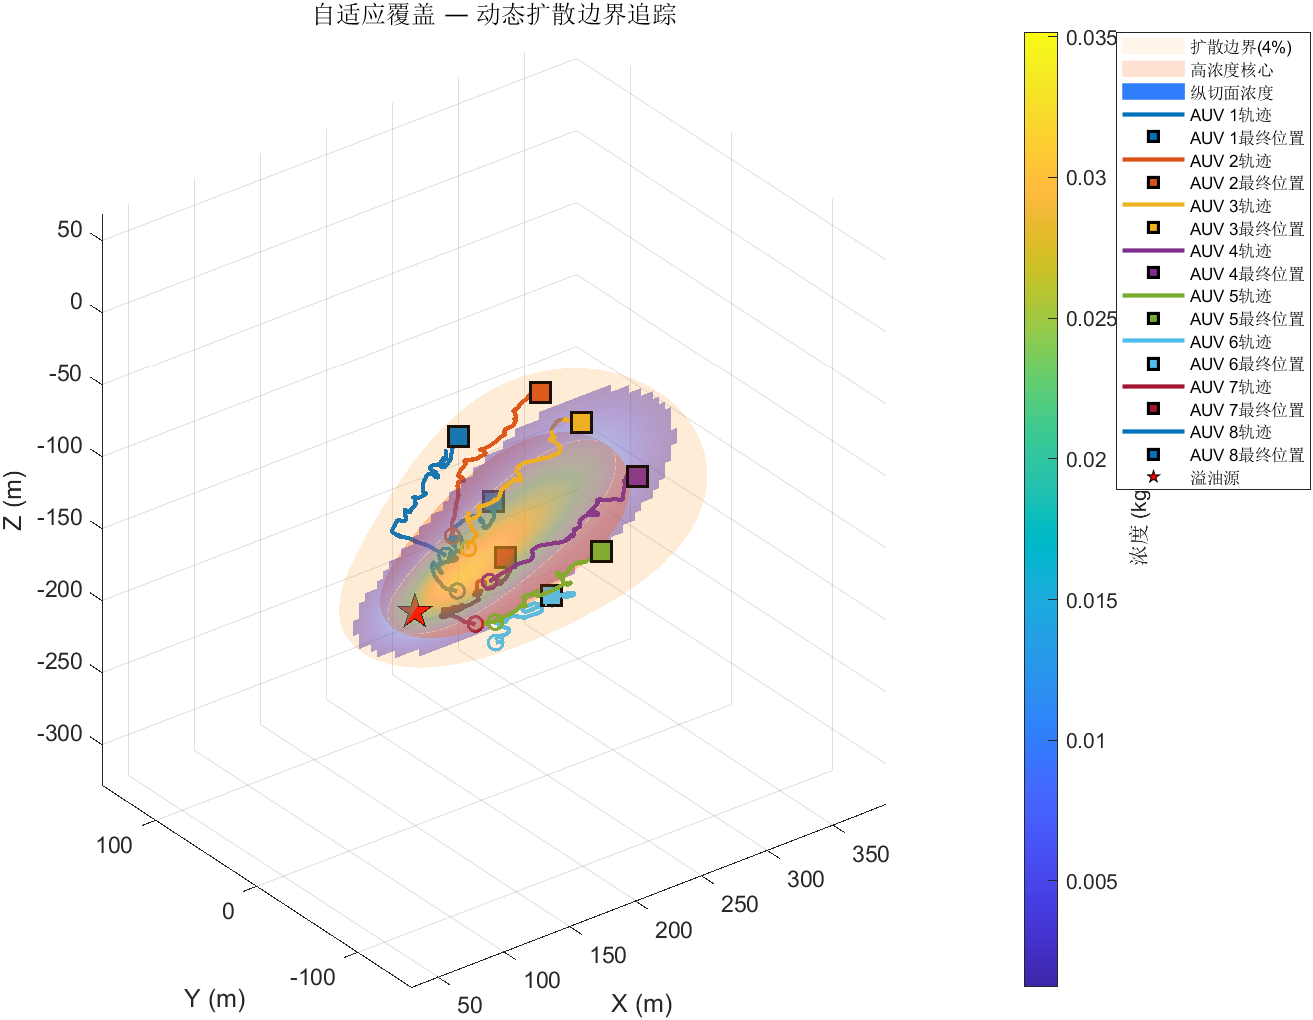
\includegraphics[width=\linewidth]{figures/step8_plume_agents_tracking.png}
\caption{三维溢油羽流与AUV轨迹}
\label{fig:plume}
\end{figure}

图\ref{fig:voronoi}展示了三维Voronoi透明覆盖区域。不同颜色表示不同AUV负责的三维体积区域，说明本文方法不是二维表面覆盖。

\begin{figure}[htbp]
\centering
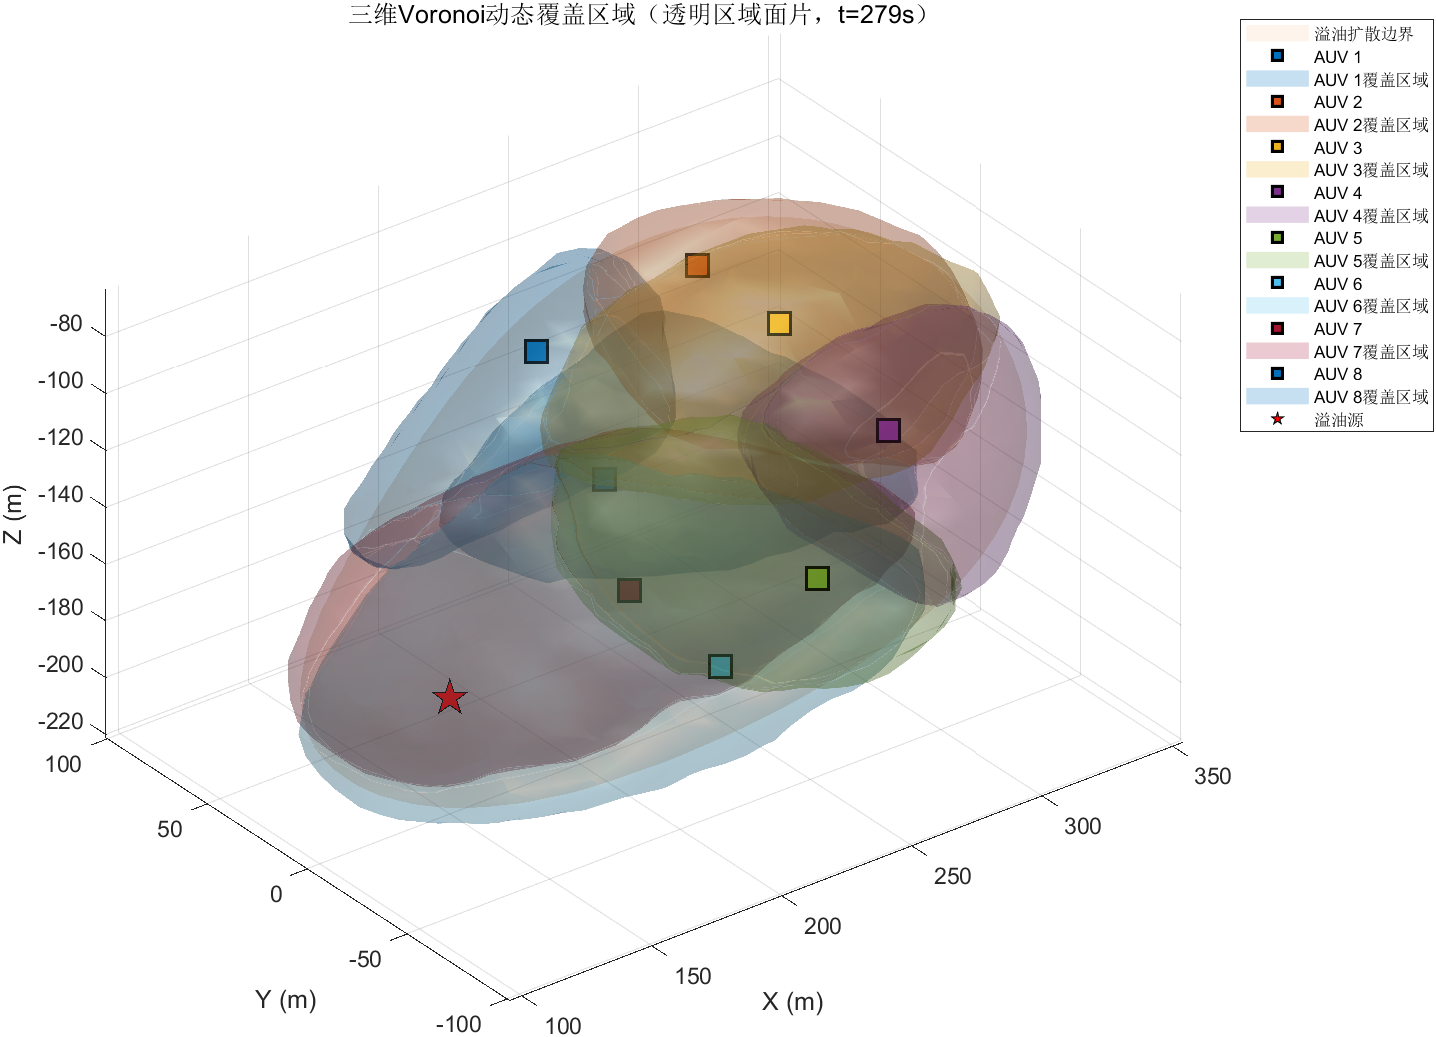
\includegraphics[width=\linewidth]{figures/step8_voronoi_3d.png}
\caption{三维Voronoi覆盖区域}
\label{fig:voronoi}
\end{figure}

图\ref{fig:H}展示覆盖质量对比。Standard CVT最终覆盖代价较低，但其原因是AUV向浓度核心区聚集，牺牲了边界监测能力。

\begin{figure}[htbp]
\centering
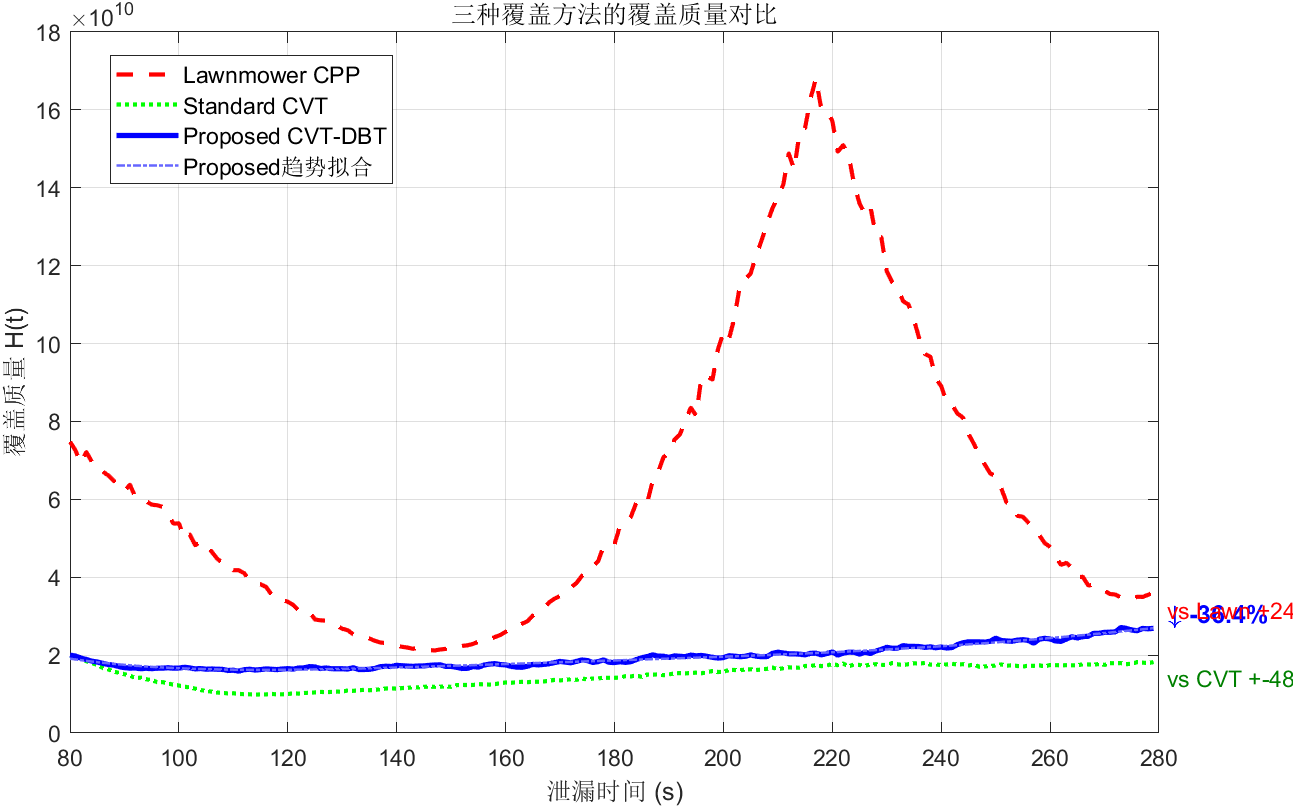
\includegraphics[width=\linewidth]{figures/step8_coverage_quality.png}
\caption{覆盖质量对比}
\label{fig:H}
\end{figure}

图\ref{fig:metrics}展示动态覆盖率和边界RMSE对比，表\ref{tab:results}给出关键指标。

\begin{figure}[htbp]
\centering
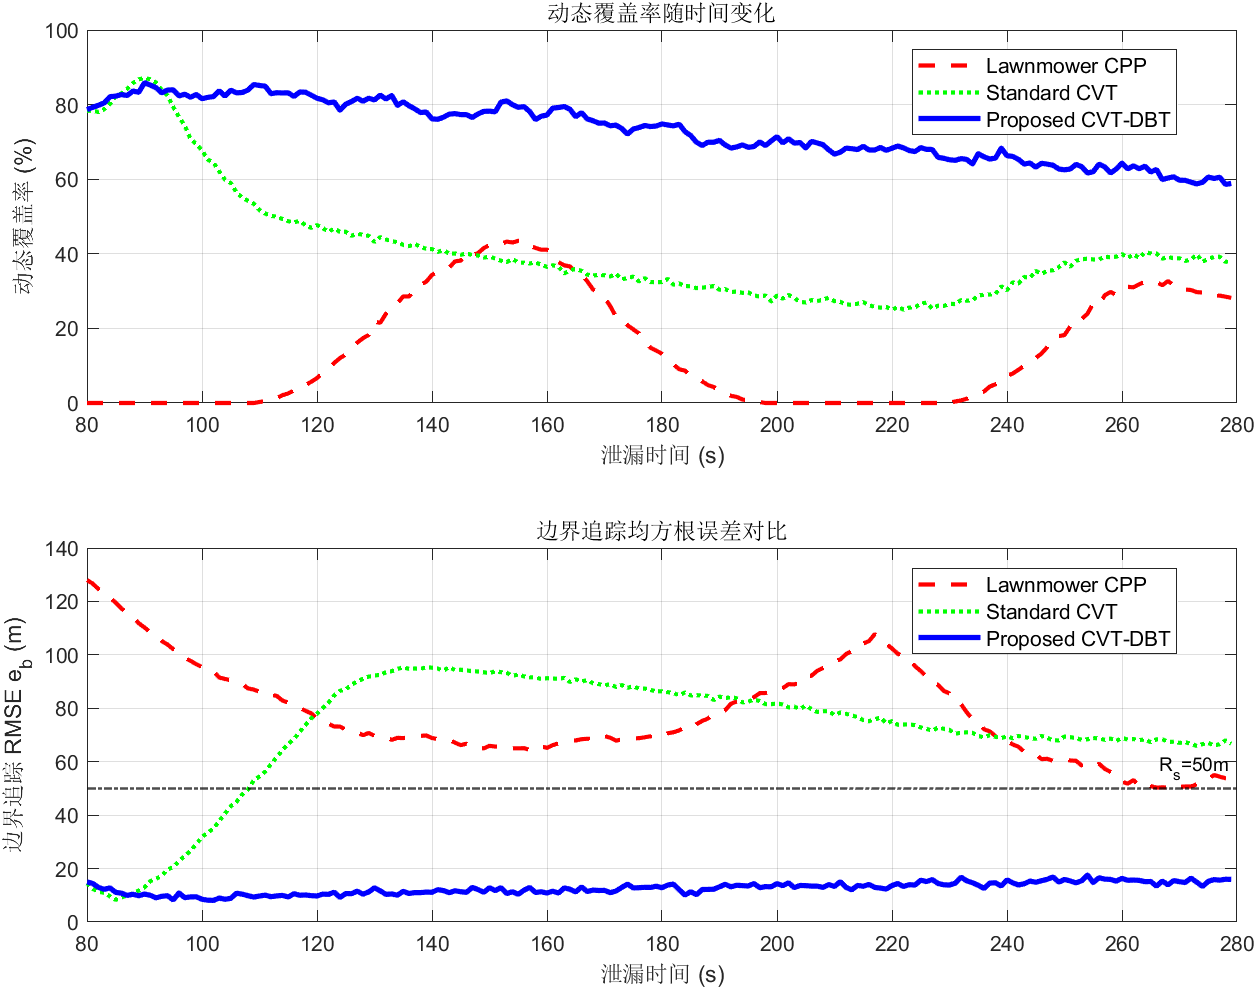
\includegraphics[width=\linewidth]{figures/step8_coverage_metrics.png}
\caption{动态覆盖率与边界追踪RMSE对比}
\label{fig:metrics}
\end{figure}

\begin{table}[htbp]
\caption{三种方法关键指标对比}
\label{tab:results}
\centering
\begin{tabular}{llll}
\toprule
方法 & $\mathcal{H}(T)$ & $CR(T)$ & RMSE\\
\midrule
CVT-DBT & $2.687\times10^{10}$ & 58.86\% & 15.94 m\\
Standard CVT & $1.821\times10^{10}$ & 38.24\% & 66.75 m\\
Lawnmower CPP & $3.606\times10^{10}$ & 28.20\% & 54.10 m\\
\bottomrule
\end{tabular}
\end{table}

结果表明，所提CVT-DBT方法相比Standard CVT将边界RMSE由66.75 m降低至15.94 m，降低约76.1\%。同时，动态覆盖率由38.24\%提升至58.86\%。这说明动态边界追踪项和空间均衡分配机制能够有效缓解集群塌陷问题。

图\ref{fig:control}展示AUV速度曲线。所有AUV速度均满足 $v_{\max}=3.5$ m/s约束，且速度变化平滑，说明控制输入具有工程可实现性。

\begin{figure}[htbp]
\centering
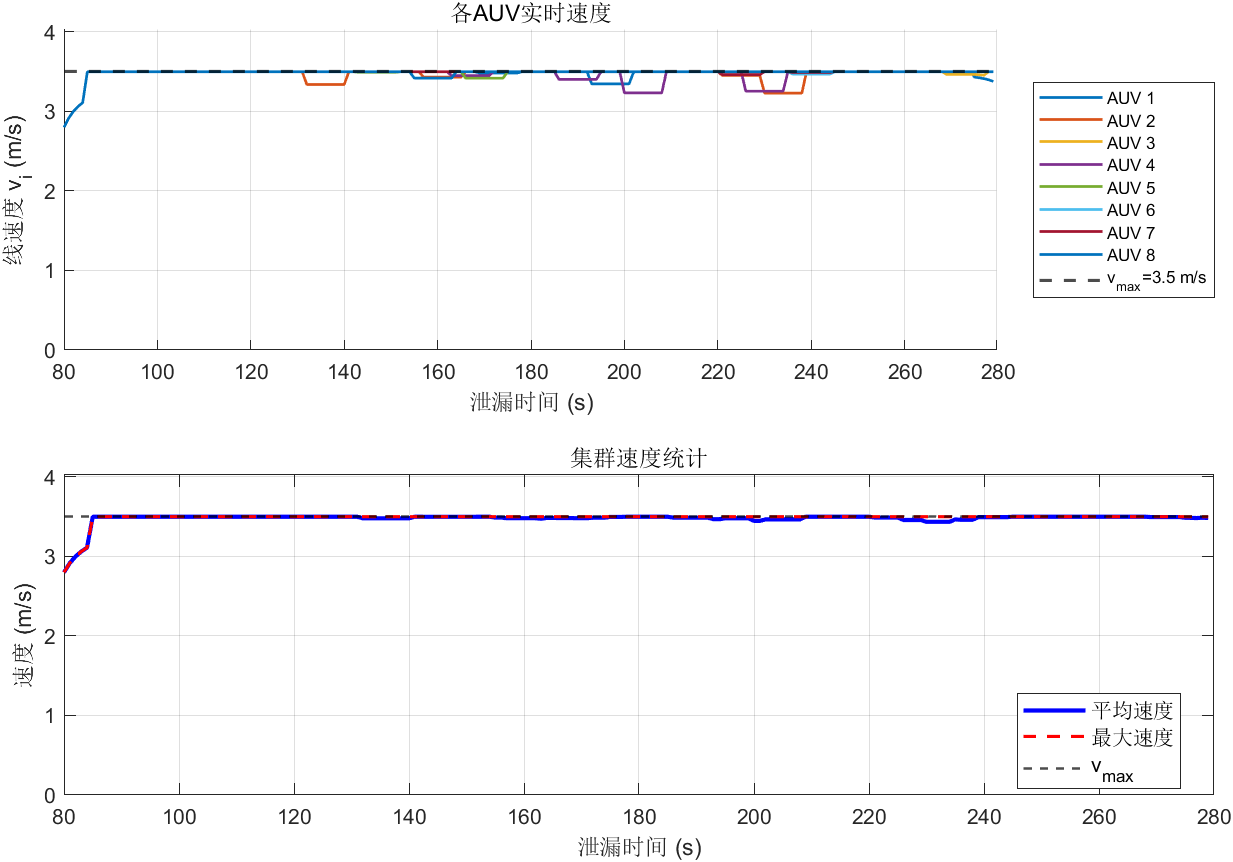
\includegraphics[width=\linewidth]{figures/step8_control_input.png}
\caption{AUV控制输入速度曲线}
\label{fig:control}
\end{figure}

\section{结论}
本文面向水下持续泄漏溢油监测问题，提出了一种融合三维Voronoi自适应覆盖与动态边界追踪的多AUV协同监测方法。首先，建立了考虑主流输运、各向异性扩散、浮力上升和自然衰减的持续泄漏三维羽流模型。其次，构造三维体积Voronoi划分与密度加权质心，实现AUV对高污染风险区域的自适应覆盖。进一步地，本文引入动态边界采样与空间均衡分配机制，设计包含质心反馈、质心速度前馈、边界追踪和分散项的速度受限控制律。

仿真实验表明，Standard CVT虽然获得较低覆盖代价，但存在明显集群塌陷，最终动态覆盖率仅为38.24\%，边界RMSE为66.75 m。所提CVT-DBT方法在覆盖代价适度增加的前提下，将动态覆盖率提升至58.86\%，并将边界RMSE降低至15.94 m，同时满足AUV速度约束。未来工作将进一步考虑AUV避碰、通信受限、复杂海底地形和控制障碍函数安全约束。

\begin{thebibliography}{00}

\bibitem{cortes2004coverage}
J. Cortés, S. Martínez, T. Karatas, and F. Bullo, ``Coverage control for mobile sensing networks,'' \textit{IEEE Transactions on Robotics and Automation}, vol. 20, no. 2, pp. 243--255, 2004, doi: 10.1109/TRA.2004.824698.

\bibitem{du2006lloyd}
Q. Du, M. Emelianenko, and L. Ju, ``Convergence of the Lloyd algorithm for computing centroidal Voronoi tessellations,'' \textit{SIAM Journal on Numerical Analysis}, vol. 44, no. 1, pp. 102--119, 2006, doi: 10.1137/040617364.

\bibitem{pierson2019generalized}
A. Pierson, L. C. Figueiredo, L. C. A. Pimenta, and M. Schwager, ``Generalized coverage control for time-varying density functions,'' in \textit{Proc. European Control Conference}, 2019, pp. 993--998, doi: 10.23919/ECC.2019.8795637.

\bibitem{zhang2020oil}
H. Zhang, Y. Li, X. Wang, and others, ``The influence of oil leaking rate and ocean current velocity on the migration and diffusion of underwater oil spill,'' \textit{Scientific Reports}, vol. 10, Art. no. 7983, 2020, doi: 10.1038/s41598-020-66046-1.

\bibitem{fingas2022overview}
M. Fingas, ``An overview of oil spill modeling and simulation for surface and subsurface applications,'' \textit{Eng}, vol. 3, no. 4, pp. 631--645, 2022, doi: 10.3390/eng3040029.

\end{thebibliography}

\end{document}
